%------------------------------------------------------------
%------------------------------------------------------------
%------------------------------------------------------------
\chapter{Arbres binaires de recherche}
%--------------------------------------------------------------------------
%--------------------------------------------------------------------------
%--------------------------------------------------------------------------
\section{Introduction}
%--------------------------------
%--------------------------------

Nous allons, dans ce chapitre, utiliser les arbres binaires ; leur principal intérêt est que chaque nœud est accessible par un chemin de longueur $h$ au plus depuis la racine  où $h$ est la hauteur de l'arbre. De plus la hauteur peut être aussi petite que $\log_2(n)$ où $n$ est la taille de l'arbre (le nombre de nœuds).

\medskip

Il reste alors deux étapes pour utiliser pleinement cette caractéristique.
%--------------------------------
\begin{itemize}
\item Comment savoir où chercher dans l'arbre ?

Il faudra ajouter une propriété supplémentaire, c'est l'objet de ce chapitre.

\item Comment assurer une hauteur qui reste de l'ordre de $\log_2(n)$ ?

Il faudra maintenir des arbres équilibrés : arbres AVL, arbres rouge-noir, arbres 2-3, \dots

Ce sera l'objet d'un T.P.
\end{itemize}

Dans ce chapitre les nœuds porteront une variable d'un type qui peut être composé.

On supposera donnée une fonction \type{cle} qui associe un entier à chaque valeur.
%--------------------------------
\begin{lstlisting}
cle 'a  -> bool
\end{lstlisting} 
%--------------------------------
On imposera que les clés doivent être distinctes dans l'arbre. ; autrement dit la restriction de la fonction \type{cle} aux valeurs de l'arbre doit être injective.

Dans les exemple, les variables seront entières et on peut écrire
%--------------------------------
\begin{lstlisting}
let cle x = x;;
\end{lstlisting} 
%--------------------------------
\newpage
%--------------------------------
\section{Arbres binaires de recherche}
%--------------------------------
%--------------------------------
\subsection{Définition}
%--------------------------------
\begin{defin}{Arbre binaire de recherche (ABR)}{abr}
Un arbre binaire de recherche est un arbre binaire tel que,  pour tout nœud $x$,  les clés des éléments du fils gauche sont strictement inférieures à la clé de $x$ et les clés des éléments du fils droit sont strictement supérieures à la clé de $x$.
\end{defin}

{\bf Exemple}

\begin{center}
\begin{tikzpicture}[level distance =2cm,scale=0.8]
  \tikzstyle{level 1}=[sibling distance =5cm]
  \tikzstyle{level 2}=[sibling distance =3 cm]
  \tikzstyle{level 3}=[sibling distance =2 cm]
  \tikzstyle{every node}=[circle,draw]
  \node  {$22$}
   child {node{$13$}
           child {node{$11$}}
           child {node{$18$}
                  child {node{$16$}}
                  child [fill=none] {edge from parent[draw=none]}
                 }
        }
  child {node {$28$}
         child [fill=none] {edge from parent[draw=none]}
         child {node{$31$}}
        };
\end{tikzpicture}
\end{center}

La déclaration du type est la même que dans le cas d'un arbre binaire classique. Il faut vérifier soi--même que les clés sont distinctes et dans le bon ordre.

%--------------------------------
\begin{lstlisting}
type 'a abr = Vide | Noeud of ('a abr*'a*'a abr);; 
\end{lstlisting} 
%--------------------------------
On étudiera des arbres de type \type{int} dans les illustrations du cours.

On ne dessinera en général pas les feuilles vides.
%--------------------------------
%--------------------------------
\subsection{Recherche}
%--------------------------------
Une fonction de base est la recherche d'un élément dans un arbre : on renvoie un booléen indiquant s'il existe un élément de clé donnée dans l'arbre. Pour cela on ''descend'' dans l'arbre en choisissant le fils gauche ou le fils droit selon que la valeur à chercher est inférieure ou supérieure au la clé de la racine. On remarque que c'est le principe de la recherche par dichotomie

On parcourt ainsi (partiellement) une branche de l'arbre.

\medskip

Si on aboutit à la valeur, c'est qu'elle est dans l'arbre. Par exemple, si on cherche 18
\begin{center}
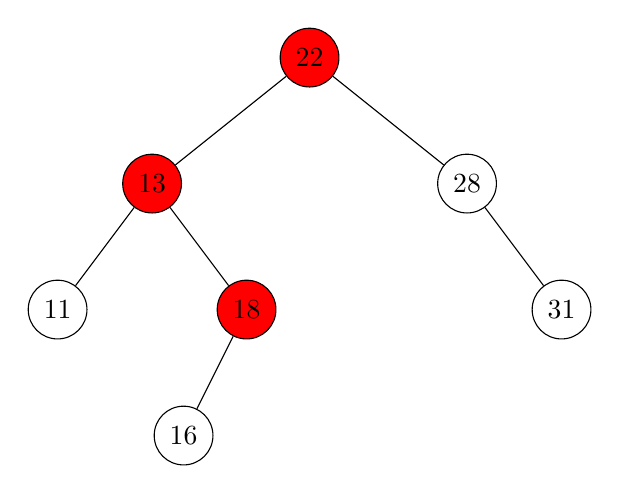
\begin{tikzpicture}[level distance =2cm,scale=0.8]
  \tikzstyle{level 1}=[sibling distance =5cm]
  \tikzstyle{level 2}=[sibling distance =3 cm]
  \tikzstyle{level 3}=[sibling distance =2 cm]
  \tikzstyle{every node}=[circle,draw]
  \node[fill=red] {$22$}
   child {node[fill=red]{$13$}
           child {node{$11$}}
           child {node[fill=red]{$18$}
                  child {node{$16$}}
                  child [fill=none] {edge from parent[draw=none]}
                 }
        }
  child {node{$28$}
         child [fill=none] {edge from parent[draw=none]}
         child {node{$31$}}
        };
\end{tikzpicture}
\end{center}

Par contre, si on aboutit à une feuille, c'est que la valeur n'est pas dans l'arbre. 

Par exemple si on cherche 23 :
\begin{center}
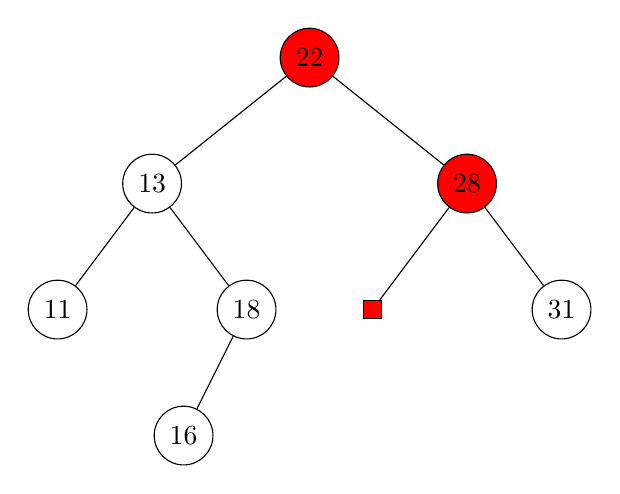
\begin{tikzpicture}[level distance =2cm,scale=0.8]
  \tikzstyle{level 1}=[sibling distance =5cm]
  \tikzstyle{level 2}=[sibling distance =3 cm]
  \tikzstyle{level 3}=[sibling distance =2 cm]
  \tikzstyle{every node}=[circle,draw]
  \node[fill=red] {$22$}
   child {node{$13$}
           child {node{$11$}}
           child {node{$18$}
                  child {node{$16$}}
                  child [fill=none] {edge from parent[draw=none]}
                 }
        }
  child {node[fill=red]{$28$}
         child {node[rectangle, draw, fill=red] {}}
         child {node{$31$}}
        };
\end{tikzpicture}
\end{center}

%--------------------------------
\begin{code}{Recherche dans un arbre binaire de recherche}{ABRsearch}
\begin{lstlisting}
let rec chercher k arbre = 
   match arbre with
   |Vide -> false
   |Noeud(g, r, d) when cle r = k -> true
   |Noeud(g, r, d) when k < cle r -> chercher k g
   |Noeud(g, r, d) -> chercher k d;;
\end{lstlisting}
\end{code}
%--------------------------------
%--------------------------------
\subsection{Analyse de la recherche}
%--------------------------------
%--------------------------------
Nous allons établir la terminaison, la preuve et la complexité en même temps en séparant les cas où la clé recherchée est ou n'est pas dans l'arbre.  La complexité est comptée en nombre de comparaisons.

%--------------------------------
\subsubsection{Absence de la clé}
%--------------------------------
 Si la clé n'est pas dans l'arbre, chaque appel de la fonction à partir d'un sous-arbre non vide fera un appel à la fonction avec un des deux fils. Ainsi la hauteur de l'arbre en paramètre de la fonction diminue strictement à chaque appel. Comme la hauteur ne peut être inférieure à -1 le nombre d'appel est fini et on aboutit à un appel \type{chercher x Vide} qui renvoie \type{false}.
 
L'algorithme termine en renvoyant la bonne réponse. De plus la diminution  d'au moins 1 de la hauteur à chaque appel récursif montre que le nombre d'appel est au plus $h+1$. Comme on fait 2 comparaisons à chaque appel sauf pour le cas de l'arbre vide la complexité en nombre de comparaisons est majorée par $2(h+1)$ ($h$ est la hauteur de l'arbre).

%--------------------------------
\subsubsection{Clé présente}
%--------------------------------
 En s'inspirant du résultat ci-dessus on note ${\cal P}_h$ la propriété :

\begin{defin}{Propriété ${\cal P}_h$}{}
Pour tout arbre \type{a} de hauteur $h$ et pour toute clé \type{k} apparaissant dans l'arbre 
\type{chercher k a} renvoie \type{true} avec $2h+1$ comparaisons au plus
\end{defin}

On notera que l'arbre est non vide car il contient au moins le nœud de clé $k$, ainsi $h\ge 0$.

\begin{description}
\item[Initialisation] ${\cal P}_0$ est vraie car un arbre de hauteur 0 qui au moins une clé ne peut être qu'un arbre de la forme 
\type{Noeud(Vide, r,  Vide)}  avec \type{cle x = k} :  dans ce cas la fonction renvoie \type{true} après 1 comparaison.

\item[Progression] On suppose que  ${\cal P}_m$ est vraie pour tout $m< h$ ($h\ge 1$). 

\type{a = Noeud(g, r, d)} est un arbre de hauteur $h$ qui contient  un élément de clé \type{k}.

\begin{itemize}
\item Si on a \type{cle r = k}, la fonction \type{chercher k a} renvoie \type{true} avec 1 comparaison.

\item Si on a \type{k <cle r} alors l'élément de clé $k$ ne peut pas être \type{d} donc \type{g} contient \type{k} et est de hauteur $h-1$ au plus.

 \type{chercher k a} effectue 2 comparaisons puis appelle \type{chercher k g} qui, d'après l'hypothèse de récurrence, renvoie \type{true} après $2(h-1)+1$ comparaisons au plus. 
 
 Ainsi \type{chercher k a} renvoie \type{true} avec $2h-1+2$ comparaisons au plus.
 
\item De même si on a \type{cle r < k} alors \type{d} contient la clé \type{k}  et \type{chercher k a} renvoie \type{true} avec $2h-1+2$ comparaisons au plus.
\end{itemize}
\item[Conclusion] La propriété est prouvée par récurrence.

\end{description}

 On a ainsi prouvé que l'algorithme termine dans tous les cas, qu'il renvoie la réponse exacte et que la complexité est majorée par $2h+2$, c'est un ${\cal O}(h)$.
%--------------------------------
%--------------------------------
\subsection{Insertion aux feuilles}
%--------------------------------
Lorsque l'on cherche un élément qui n'est pas dans l'arbre, on aboutit à une feuille ; on peut alors remplacer la feuille par un nœud terminal.

Si l'élément était déjà présent, on ne change rien.

\medskip

Ici encore la complexité est proportionnelle au nombre d'appels récursifs effectués donc est de la forme ${\cal O}(h)$ où $h$ est la hauteur de l'arbre.

{\bf Exemple} : on ajoute 25 à l'exemple initial :

\begin{center}
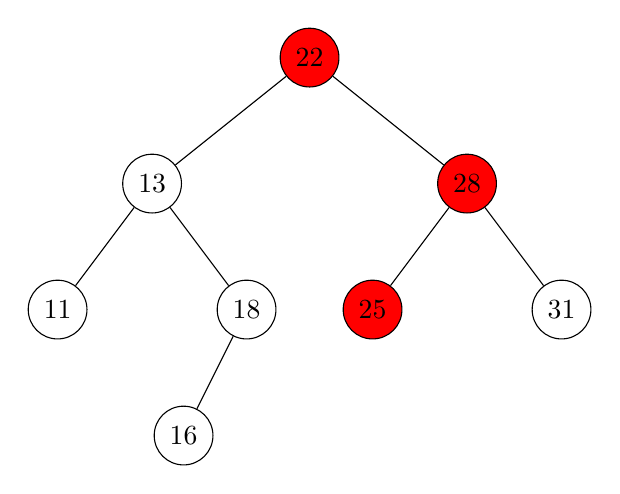
\begin{tikzpicture}[level distance =2cm,scale=0.8]
  \tikzstyle{level 1}=[sibling distance =5cm]
  \tikzstyle{level 2}=[sibling distance =3 cm]
  \tikzstyle{level 3}=[sibling distance =2 cm]
  \tikzstyle{every node}=[circle,draw]
  \node[fill=red] {$22$}
   child {node{$13$}
           child {node{$11$}}
           child {node{$18$}
                  child {node{$16$}}
                  child [fill=none] {edge from parent[draw=none]}
                 }
        }
  child {node[fill=red]{$28$}
              child {node[fill=red]{$25$}}
              child {node{$31$}}
        };
\end{tikzpicture}
\end{center}
%--------------------------------
\begin{code}{Insertion aux feuilles}{ABRleaf}
\begin{lstlisting}
let rec insertionF x arbre = 
   match arbre with
   |Vide -> Noeud(Vide, x,  Vide)
   |Noeud(g, r d) when cle r = cle x-> Noeud(g, x, d)
   |Noeud(g, r, d) when cle x = cle r
                   -> Noeud((insertionF x  g), r, d)
   |Noeud(g, r, d) -> Noeud(g, r, (insertionF x  d));;
\end{lstlisting}
\end{code}
%--------------------------------
% %--------------------------------
% \subsection{Insertion à la racine}
% %--------------------------------
% On peut aussi choisir d'insérer un nouveau nœud en le plaçant à la racine.

% Pour cela on va couper l'arbre en deux parties regroupant les nœuds inférieurs à la nouvelle clé et ceux qui sont supérieurs.
% La récursivité permet de le faire avec un coût minimum c'est-à-dire proportionnel à la hauteur et non à la taille.


% Le dernier arbre construit est coupé par 17 :


% \begin{center}
% \begin{tikzpicture}
% \tikzstyle{every node}=[circle,draw,minimum size=8mm]
% \node at (0,0) (r) {22};
% \node at (-2.5,-1.5) (fg) {13};
% \node at (2.5,-1.5) (fd) {28};
% \node at (-4,-2.8) (fgg) {11};
% \node at (-1,-2.8) (fgd) {18};
% \node at (1,-2.8) (fdg) {25};
% \node at (4,-2.8) (fdd) {31};
% \node at (-2,-4) (fgdg) {16};
% \draw (r) -- (fd)
%      (fg) -- (fgg)
%      (fd) -- (fdd)
%      (fd) -- (fdg);
% \draw [red,dashed]
%       (r) -- (fg)
%      (fg) -- (fgd)
%     (fgd) -- (fgdg);
% \draw[>-<,thick, red] (-1.5,0) --  (-1.5,-4.5);
% \end{tikzpicture}
% \end{center}

% On reconstruit deux arbres : 

% \begin{center}
% \begin{tikzpicture}
% \tikzstyle{every node}=[circle,draw,minimum size=8mm]
% \node at (0,0) (r) {22};
% \node at (-5,0) (fg) {13};
% \node at (1.5,-1.5) (fd) {28};
% \node at (-6.5,-1.5) (fgg) {11};
% \node at (-1.5,-1.5) (fgd) {18};
% \node at (0.5,-2.8) (fdg) {25};
% \node at (2.5,-2.8) (fdd) {31};
% \node at (-3.5,-1.5) (fgdg) {16};
% \draw (r) -- (fd)
%       (r) -- (fgd)
%      (fg) -- (fgg)
%      (fg) -- (fgdg)
%      (fd) -- (fdd)
%      (fd) -- (fdg);
% \end{tikzpicture}
% \end{center}

% On peut alors ajouter le nœud 17 à la racine.

% \begin{center}
% \begin{tikzpicture}
% \tikzstyle{every node}=[circle,draw,minimum size=8mm]
% \node[fill=red] at (-2.5,1.7) (r0) {17};
% \node at (0,0) (r) {22};
% \node at (-5,0) (fg) {13};
% \node at (1.5,-1.5) (fd) {28};
% \node at (-6.5,-1.5) (fgg) {11};
% \node at (-1.5,-1.5) (fgd) {18};
% \node at (0.5,-2.8) (fdg) {25};
% \node at (2.5,-2.8) (fdd) {31};
% \node at (-3.5,-1.5) (fgdg) {16};
% \draw (r) -- (fd)
%       (r) -- (fgd)
%      (fg) -- (fgg)
%      (fg) -- (fgdg)
%      (fd) -- (fdd)
%      (fd) -- (fdg);
% \draw[dashed]  (r0) -- (r)
%               (r0) -- (fg);
% \end{tikzpicture}\end{center}

% \medskip

% La première étape consiste à produire les deux arbres séparés par la clé de l'élément que l'on veut ajouter. Le découpage et la reconstitution se font en même temps, récursivement.

% Si la clé de la valeur est strictement inférieure à celle de la racine.

% \begin{itemize}
% \item On découpe le fils gauche avec la même valeur. On obtient deux arbres : \type{g\_inf}, l'arbre formés des nœuds du fils gauche de clé inférieure à la coupure et \type{g\_sup}.
% \begin{center}
% \begin{tikzpicture}
% \tikzstyle{every node}=[circle,draw,minimum size=8mm]
% \node at (-5,0) (fg) {13};
% \node at (-6.5,-1.5) (fgg) {11};
% \node at (-1.5,0) (fgd) {18};
% \node at (-3.5,-1.5) (fgdg) {16};
% \draw (fg) -- (fgg)
%       (fg) -- (fgdg);
% \end{tikzpicture}
% \end{center}


% \item L'arbre des nœuds inférieurs à la coupure est alors \type{g\_inf}.
% \item L'arbre des nœuds supérieurs à la coupure est formé en remplaçant le fils gauche initial par \type{g\_sup}.
% \end{itemize}

% On fait les opérations symétriques si la coupure est strictement supérieure à la racine.

% En cas d'égalité on retire la racine et on renvoie les deux fils. 

% %--------------------------------
% \placecode[force][code:rootBST]{Insertion à la racine dans un arbre binaire de recherche}{
% \startML
% let rec decoupage k a = 
%   match a with
%   |Vide -> (Vide,Vide)
%   |Noeud(g, r, d) when cle r = r -> (g, d)
%   |Noeud(g, r, d) when k < cle r
%                   -> let (gg, gd) = decoupage k g 
%                      in (gg, Noeud(gd, r, d))
%   |Noeud(g,r, d) -> let (dg, dd) = decoupage k d 
%                      in (Noeud(g, r, dg),dd);;
                
% let insertionRacine x a =
%   let (g, d)= decoupage (cle x) a 
%   in Noeud(g,x, d);;
% \stopML}

% Ici encore on remplace l'élément de l'arbre qui a une clé égale à celle de l'élément à ajouter.
% %--------------------------------
% \newpage
% %--------------------------------
% \subsection{Suppression}
% %--------------------------------
% La suppression d'un nœud demande de conserver la structure ordonnée.

% Il est relativement facile d'imaginer comment supprimer une feuille : on la remplace par l'arbre vide.

% Le cas d'un nœud interne $n$ est plus délicat. On se ramène au cas de la racine car il suffira de remplacer le sous--arbre dont $n$ est la racine par l'arbre diminué.

% Un cas simple est celui d'un nœud sans fils gauche (ou droit) : l'arbre allégé est alors simplement le fils droit (ou gauche).

% Pour ôter la racine d'un sous--arbre sans trop de modification on va choisir de le remplacer par un autre nœud de l'arbre. On choisira sa clé pour conserver la structure d'arbre binaire de recherche avec le minimum de modifications : le maximum dans le fils gauche (ou le minimum du fils droit) est un bon choix car sa clé sépare les cles restantes et on le remplace facilement par son fils gauche.

% \medskip
% On va donc opérer en 4 étapes.

% \begin{center}
% \begin{tikzpicture}
% \tikzstyle{every node}=[circle,draw,minimum size=8mm]
% \node at (-6,2)(fgg)  { 6};
% \node at (-5,3)(fg)   { 9};
% \node at (-4,0)(fgdgg){11};
% \node at (-3,1)(fgdg) {12};
% \node at (-2,0)(fgdgd){14};
% \node at (-1,2)(fgd)  {16};
% \node at ( 0,4)(r)    {17};
% \node at ( 1,2)(fdg)  {18};
% \node at ( 2,3)(fd)   {22};
% \node at ( 3,1)(fddg) {25};
% \node at ( 4,2)(fdd)  {28};
% \node at ( 5,1)(fddd) {31};
% \draw    (r) --    (fg)
%          (r) --    (fd)
%         (fg) --   (fgg)
%         (fg) --   (fgd)
%         (fd) --   (fdg)
%         (fd) --   (fdd)
%       (fgd) --  (fgdg)
%       (fdd) --  (fddg)
%       (fdd) --  (fddd)
%       (fgdg) -- (fgdgg)
%       (fgdg) -- (fgdgd);
% \end{tikzpicture}\end{center}

% \subsubsection{Enlever la racine}

% \begin{center}
% \begin{tikzpicture}
% \tikzstyle{every node}=[circle,draw,minimum size=8mm]
% \node at (-6,2)(fgg)  { 6};
% \node at (-5,3)(fg)   { 9};
% \node at (-4,0)(fgdgg){11};
% \node at (-3,1)(fgdg) {12};
% \node at (-2,0)(fgdgd){14};
% \node at (-1,2)(fgd)  {16};
% %\node at ( 0,4)(r)    {17};
% \node at ( 1,2)(fdg)  {18};
% \node at ( 2,3)(fd)   {22};
% \node at ( 3,1)(fddg) {25};
% \node at ( 4,2)(fdd)  {28};
% \node at ( 5,1)(fddd) {31};
% \draw   (fg) --   (fgg)
%         (fg) --   (fgd)
%         (fd) --   (fdg)
%         (fd) --   (fdd)
%       (fgd) --  (fgdg)
%       (fdd) --  (fddg)
%       (fdd) --  (fddd)
%       (fgdg) -- (fgdgg)
%       (fgdg) -- (fgdgd);
% \end{tikzpicture}\end{center}

% \subsubsection{Calculer la clé maximale du fils gauche}

% On cherche récursivement le fils droit sans fils droit.

% \begin{center}
% \begin{tikzpicture}
% \tikzstyle{every node}=[circle,draw,minimum size=8mm]
% \node at (-6,2)(fgg)  { 6};
% \node at (-5,3)(fg)   { 9};
% \node at (-4,0)(fgdgg){11};
% \node at (-3,1)(fgdg) {12};
% \node at (-2,0)(fgdgd){14};
% \node[fill=red] at (-1,2)(fgd)  {16};
% \node at ( 1,2)(fdg)  {18};
% \node at ( 2,3)(fd)   {22};
% \node at ( 3,1)(fddg) {25};
% \node at ( 4,2)(fdd)  {28};
% \node at ( 5,1)(fddd) {31};
% \draw   (fg) --   (fgg)
%         (fd) --   (fdg)
%         (fd) --   (fdd)
%       (fdd) --  (fddg)
%       (fdd) --  (fddd)
%       (fgdg) -- (fgdgg)
%       (fgdg) -- (fgdgd)
%         (fg) --   (fgd)
%       (fgd) --  (fgdg);
% \end{tikzpicture}\end{center}

% \subsubsection{Reconstituer le fils gauche}

% Si $T$ est le sous--arbre du fils gauche dont la clé est maximale alors il n'a pas de fils droit (qui, sinon, aurait des clés supérieures)~; le fils gauche de $T$ remplace  $T$.

% \begin{center}
% \begin{tikzpicture}
% \tikzstyle{every node}=[circle,draw,minimum size=8mm]
% \node at (-6,2)(fgg)  { 6};
% \node at (-5,3)(fg)   { 9};
% \node at (-4,1)(fgdgg){11};
% \node at (-3,2)(fgdg) {12};
% \node at (-2,1)(fgdgd){14};
% \node at (-1,2)(fgd)  {16};
% \node at ( 1,2)(fdg)  {18};
% \node at ( 2,3)(fd)   {22};
% \node at ( 3,1)(fddg) {25};
% \node at ( 4,2)(fdd)  {28};
% \node at ( 5,1)(fddd) {31};
% \draw   (fg) --   (fgg)
%         (fd) --   (fdg)
%         (fd) --   (fdd)
%       (fdd) --  (fddg)
%       (fdd) --  (fddd)
%       (fgdg) -- (fgdgg)
%       (fgdg) -- (fgdgd);
% \draw[dashed](fg) --  (fgdg);
% \end{tikzpicture}\end{center}
% \subsubsection{Reconstruire l'arbre}

% \begin{center}
% \begin{tikzpicture}
% \tikzstyle{every node}=[circle,draw,minimum size=8mm]
% \node at (-6,2)(fgg)  { 6};
% \node at (-5,3)(fg)   { 9};
% \node at (-4,1)(fgdgg){11};
% \node at (-3,2)(fgdg) {12};
% \node at (-2,1)(fgdgd){14};
% \node at (-1,4)(fgd)  {16};
% \node at ( 0,2)(fdg)  {18};
% \node at ( 1,3)(fd)   {22};
% \node at ( 2,1)(fddg) {25};
% \node at ( 3,2)(fdd)  {28};
% \node at ( 4,1)(fddd) {31};
% \draw   (fg) --   (fgg)
%         (fg) --  (fgdg)
%         (fd) --   (fdg)
%         (fd) --   (fdd)
%       (fdd) --  (fddg)
%       (fdd) --  (fddd)
%       (fgdg) -- (fgdgg)
%       (fgdg) -- (fgdgd)
%       (fgd) -- (fg)
%       (fgd) -- (fd);
% \end{tikzpicture}\end{center}

% On peut écrire les fonctions correspondantes

% %--------------------------------
% \begin{lstlisting}
% let rec maxArbre arbre = 
%   match arbre with
%   |Vide -> failwith "Arbre vide"
%   |Noeud(g, r, Vide) -> r
%   |Noeud(g, r, d) -> maxArbre d;;
% \end{lstlisting}
% %--------------------------------
% \begin{lstlisting}
% let rec suppressionMax arbre = 
%   match arbre with
%   |Vide -> failwith "Arbre vide"
%   |Noeud(g, r, Vide) -> g
%   |Noeud(g, r, d) -> Noeud(g, r, suppressionMax d);;
% \end{lstlisting}
% %--------------------------------
% \placecode[force][code:suppRootBST]{Suppression de la racine dans un arbre binaire de recherche}{
% \startML
% let suppressionRacine arbre = 
%   match arbre with
%   |Vide -> Vide
%   |Noeud(Vide, r, d) -> d
%   |Noeud(g, r, d) ->  let  y = maxArbre g in
%                       Noeud(suppressionMax g, y, d);;
% \stopML}
% %--------------------------------

% On peut alors revenir au cas général.

% %--------------------------------
% \placecode[force][code:suppBST]{Suppression d'un nœud dans un arbre binaire de recherche}{
% \startML
% let rec suppression k arbre = 
%   match arbre with
%   |Vide -> Vide
%   |Noeud(g, r, d) when cle r = k 
%                      -> suppressionRacine arbre
%   |Noeud(g, r, d) when k < cle r 
%                      -> Noeud((suppression k g), r, d)
%   |Noeud(g, r, d) -> Noeud(g, r, (suppression k d));;
% \stopML}
% %--------------------------------
% \newpage
% %--------------------------------
% \section{Application : dictionnaires}
% %--------------------------------
% %--------------------------------

% Lors de l'étude des structures abstraites nous avons définis les dictionnaires (ou tableaux associatifs) qui sont des structures de données abstraites où l'on stocke des éléments munis d'une clé.

% On travaillera donc  avec des éléments d'un type \type{'a} pour lesquels lae fonction \type{cle : 'a -> int} qui associe un indice unique à chaque élément est {\bf injective} .

% Le type abstrait doit définir les fonctions :
% %--------------------------------
% \begin{itemize}
% \item \type{dictionnaireVide : unit -> 'a dict}, qui construit un dictionnaire vide,
% \item \type{insertion : 'a -> 'a dict -> 'a dict}, qui insère un élément dans le dictionnaire,
% \item \type{defini : int -> 'a dict -> bool}, qui teste si une clé correspond à une entrée,
% \item \type{valeur : int -> 'a dict -> 'a}, qui retrouve, s'il existe, l'élément du dictionnaire correspondant à une clé donnée.
% \item \type{retrait : int -> 'a dict -> 'a dict}, qui élimine un élément défini par sa clé.
% \end{itemize}
% %--------------------------------
% On remarquera que les fonctions ci-dessus correspondent à un type de données persistant : on conserve les dictionnaires et l'ajout ou le retrait d'un élément crée un nouveau dictionnaire.

% \medskip

% Nous avons utilisé des tables de hachages pour implémenter cette structure : les différentes fonctions sont alors très efficaces. Cependant il est difficile dans ce cas d'énumérer les éléments, ou ceux dont les clés sont dans un intervalle. De plus le type n'est pas persistant.

% \medskip

% On peut utiliser la structure d'arbre binaire de recherche.

% Dans l'exemple les éléments seront  des couples $(a,b)$ où $a$ est la clé.

% \medskip

% {\bf Exemple}
% %--------------------------------
% \begin{center}
% \begin{tikzpicture}[level distance =15mm]
%   \tikzstyle{level 1}=[sibling distance =4cm]
%   \tikzstyle{level 2}=[sibling distance =3cm]
%   \tikzstyle{level 3}=[sibling distance =2cm]
%   \tikzstyle{every node}=[rectangle,draw, rounded corners]
%   \node {$22$, "léa''}
%   child {node{$13$, "tom"}
%           child {node{$11$, "jim"}}
%           child {node{$18$, "abe"}
%                   child {node{$16$, "ève"}}
%                   child [fill=none] {edge from parent[draw=none]}
%                  }
%         }
%   child {node{$28$,"jo"}
%           child [fill=none] {edge from parent[draw=none]}
%           child {node{$31$, "ida"}}
%         };
% \end{tikzpicture}
% \end{center}

% \newpage

% Les fonctions sont alors simplement des renommages.
% %--------------------------------
% \begin{lstlisting}
% let dictionnaireVide () -> Vide;;
% let insertion = insertionRacine;;
% let defini = chercher;;
% let retrait = suppression;;
% \end{lstlisting}
% %--------------------------------


% Sauf pour la valeur d'un élément en fonction de sa clé qui est une modification simple de la recherche.
% %--------------------------------
% \begin{lstlisting}

% let rec valeur k arbre = 
%   match arbre with
%   |Vide -> failwith "Il n'y a pas d'élément associé"
%   |Noeud(g, r, d) when cle r = k -> r
%   |Noeud(g, r, d) when k < cle r -> valeur k g
%   |Noeud(g, r, d) -> valeur k d;;
% \end{lstlisting}
% %--------------------------------
% \newpage
% %--------------------------------
% \section{Exercices}
% %--------------------------------
% %--------------------------------
% \startexo {\bf Une caractérisation } 

% Prouver qu'un arbre binaire est un arbre binaire de recherche si et seulement si le parcours {\bf infixe} des clés de l'arbre donne une suite strictement croissante.
% \stopexo
% %--------------------------------------------------------------------------
% \beginrep[exosABR]
% \startreponse 
% {\bf Sens inverse}

% On suppose que le parcours infixe lit les clés dans l'ordre croissant

% Pour tout sous--arbre les clés du fils gauche sont lues par le parcours infixe avant la clé de la racine donc, comme le parcours est croissant, les clés du fils gauche sont inférieures à celle de la racine. 

% De même les clés du fils droit sont supérieures à celle de la racine.

% L'arbre est donc bien un A.B.R.

% {\bf Sens direct}


% On vérifie la réciproque par récurrence sur la hauteur.

% \begin{itemize}
% \item C'est évident pour un sous--arbre de hauteur 0.

% \item Si c'est vrai pour tous les arbres de hauteur $p$ au plus.
% Les  fils droit et gauche  d'un arbre de hauteur $p+1$ ont une hauteur inférieure ou égale à $p$. Le parcours infixe de $T$ se fait en parcourant le fils gauche, qui donne des clés croissantes par hypothèse de récurrence, puis en lisant la clé de la racine, supérieure aux précédentes, puis en parcourant le fils droit, toujours en croissant.

% Le parcours infixe est croissant.

% \end{itemize}
% \stopreponse
% \endrep

% %--------------------------------------------------------------------------
% %--------------------------------------------------------------------------
% \startexo{\bf Parcours de recherche}

% On suppose que tous les nombres de 1 à 800 sont les clés d'un 
% arbre binaire de recherche. Parmi les suites suivantes lesquelles ne peuvent pas être les clés d'un parcours de recherche de 417 ?

% \begin{itemize}

% \item 222, 457, 122, 217, 417

% \item 601, 403, 555, 408, 523, 411, 466, 417

% \item 601, 403, 555, 408, 563, 411, 466, 417

% \item 901, 403, 555, 411, 466, 417
% \end{itemize}

% \stopexo
% %--------------------------------------------------------------------------
% \beginrep[exosABR]
% \startreponse Le principe est que si on suit un arbre binaire de recherche $u_0, u_1, \ldots, u_p$ $u_{i+1} > u_i$ impose $u_j > u_i$ pour tout $j>i$.
% \begin{itemize}
% \item 122 n'est pas possible après 222, 457

% \item 545, 215, 333, 401, 422, 417


% \item 601, 403, 555, 408, 523, 411, 466, 417


% \item 601, 403, 555, 408, 563, 411, 466, 417


% \item 901, 403, 555, 411, 466, 417
% \end{itemize}

% \stopreponse
% \endrep
% %--------------------------------------------------------------------------
% %--------------------------------------------------------------------------
% \startexo{\bf Vérification}

% Écrire une fonction qui teste si l'arbre binaire passé en paramètre est un arbre binaire de recherche.
% \stopexo
% %--------------------------------------------------------------------------
% \beginrep[exosABR]
% \startreponse \type{Noeud(g, r, d)} est un arbre binaire de recherche si 

%  \type{g} et \type{d} sont des arbres binaires de recherche,

%  le maximum des clés de \type{g} est strictement inférieur à $n$,
 
%  le minimum des clés de \type{d} est strictement supérieur à $n$.
 
%  On peut calculer les maximums et minimums par des fonctions auxiliaire mais cela revient à parcourir tout l'arbre plusieurs fois. On va tout calculer d'un coup.
 
%  L'arbre vide n'a pas de maximum, on le remplace par l'entier minimum : tout entier lui sera supérieur. De même le minimum de l'arbre vide sera choisi comme l'entier maximum.
% %--------------------------------
% \begin{lstlisting}
% let estABR arbre = 
%   let rec aux a =
%     match a with
%     |Vide -> (max_int, true, min_int)
%     |Noeud(g, r, d) -> let (m1, b1, M1) = aux g in 
%                       let (m2, b2, M2) = aux d in
%                       (m1, b1 && b2 && (M1 < cle r) && (cle r < m2), M2)
%   in let (_,b,_) = aux arbre in b;;
% \end{lstlisting}
% \stopreponse
% \endrep
% %--------------------------------------------------------------------------
% %--------------------------------------------------------------------------
% \startexo{\bf Tranche}

% Écrire une fonction \type{tranche arbre a b} qui reçoit comme paramètre un arbre binaire de recherche et deux entiers et qui renvoie un arbre binaire de recherche dont les clés son les clés de \type{arbre} comprises entre \type{a} et \type{b}.
% \stopexo
% %--------------------------------------------------------------------------
% \beginrep[exosABR]
% \startreponse 
% \begin{lstlisting}
% let rec tranche arbre a b = 
%   match arbre with
%   |Vide -> Vide
%   |Noeud(g, r, d) when cle r < a -> tranche d a b
%   |Noeud(g, r, d) when cle r > b -> tranche g a b
%   |Noeud(g, r, d) -> Noeud(tranche g a b, r, tranche d a b);;
% \end{lstlisting}
% \stopreponse
% \endrep
% %--------------------------------------------------------------------------
% %--------------------------------------------------------------------------
% \startexo{\bf Tri }

% Comment peut-on utiliser les arbres binaires de recherche pour effectuer un tri ?

% Si on admet que la hauteur moyenne d'un arbre binaire de recherche de taille $n$ est un ${\cal O}\bigl(\log_2(n)\bigr)$ déterminer la complexité, en moyenne, de ce tri.
% \stopexo
% %--------------------------------------------------------------------------
% \beginrep[exosABR]
% \startreponse L'arbre sert de réservoir qui trie tout seul les éléments qu'on lui ajoute.

% \begin{itemize}
% \item On insère (dans le désordre) les éléments à trier dans un arbre à partir de l'arbre vide.

% \item On lit l'arbre dans un parcours infixe : la liste est triée.

% \end{itemize}

% La complexité des insertions est de l'ordre de $\displaystyle \sum_{i=1}^{n-1} \ln(i)\le n\log_2(n)$.

% Le parcours est de complexité linéaire donc le tri est un ${\cal O}\bigl(n\log_2(n)\bigr)$.
% \stopreponse
% \endrep
% %--------------------------------------------------------------------------
% %--------------------------------------------------------------------------
% \startexo{\bf Fusion}

% Écrire une fonction {\tt Fusion a b} qui joint deux 
% arbres binaires de recherche ; on pourra utiliser les fonctions de coupure d'un arbre binaire de recherche.
% \stopexo
% %--------------------------------------------------------------------------
% \beginrep[exosABR]
% \startreponse Si le premier arbre est non vide on coupe le second selon la racine du premier et on ajoute les morceaux aux deux fils.
% %--------------------------------
% \begin{lstlisting}
% let rec fusion arbre1 arbre2 =
%   match arbre1 with
%   |Vide -> arbre2
%   |Noeud(g, r, d) -> let (pt, gd) = decoupage (cle r) arbre2 in
%                         Noeud(fusion g pt, r, fusion d gd);;
% \end{lstlisting}
% %--------------------------------
% \stopreponse
% \endrep
% %--------------------------------------------------------------------------
% %--------------------------------------------------------------------------
% \startexo{\bf Ancêtre commun}

% Un ancêtre commun de deux nœuds $n_1$ et $n_2$ d'un arbre homogène est un nœud dont $n_1$ et $n_2$ sont descendants ; en particulier la racine est toujours un ancêtre commun de toute paire de nœuds.

% \begin{itemize}
% \item Montrer que, pour tout entier $h$, deux nœuds $n_1$ et $n_2$ admettent au plus un ancêtre commun à la profondeur $h$.

% \medskip

% On appelle {\bf plus proche ancêtre commun}, noté PPAC,  de $n_1$ et $n_2$ leur ancêtre commun de profondeur maximale.

% D'après le résultat ci-dessus le plus proche ancêtre commun est unique.

% \medskip

% \item Prouver que les ancêtres communs de $n_1$ et $n_2$ sont les ancêtres de leur PPAC.

% \item $n_1$ et $n_2$ sont deux nœuds d'un arbre. Prouver que leur PPAC est
% \startitemize[n,joinedup]
% \item $n_1$, si $n_2$ est un descendant de $n_1$,
% \item $n_2$, si $n_1$ est un descendant de $n_2$,
% \item l'unique nœud $n$ de l'arbre tel que $n_1$ appartient au fils gauche (resp. fils droit) de $n$ et $n_2$ appartient au fils droit (resp. fils gauche) de $n$ dans les autres cas.
% \end{itemize}

% \item En déduire l'écriture d'une fonction qui permet de déterminer le PPAC de deux nœuds d'un A.B.R.
% \end{itemize}
% \stopexo
% %--------------------------------------------------------------------------
% \beginrep[exosABR]
% \startreponse 
% \begin{itemize}
% \item Deux nœuds de même profondeur définissent deux sous-arbres disjoints : ils ne peuvent donc pas être en même temps ancêtres communs de $n_1$ et $n_2$.

% \item Les ancêtres d'un d'un ancêtre commun sont des ancêtres communs, en particulier les ancêtres du PPAC sont des ancêtres communs.

% Inversement, si $n$ est un ancêtre commun de $n_1$ et $n_2$, sa profondeur $h$ est inférieure à celle du PPAC. On considère alors l'ancêtre de profondeur $h$ du PPAC ; $n'$. $n'$ est un ancêtre commun de $n_1$ et $n_2$ de même hauteur que $n$ donc $n=n'$ d'après la premieère question. Ainsi $n$ est un ancêtre du PPAC

% Les ancêtres communs sont bien les ancêtres du PPAC.

% \item On suppose que $n_1$ n'est pas un descendant de $n_2$ et $n_2$ n'est pas un descendant de $n_1$ .

% $n$ est le PPAC de $n_1$ et $n_2$, on a $n\ne n_1$ et $n \ne n_2$.

% Ainsi $n_1$ et $n_2$ appartiennent aux fils de $n$.

% S'il appartenaient au même fils celui-ci serait un ancêtre commun, ce qui contredirait la minimalité de la hauteur. Ainsi $n_1$ et $n_2$ appartiennent à des fils distincts de $n$.

% \item 
% %--------------------------------
% \begin{lstlisting}
% let rec ppac arbre p q =
%   match arbre with
%   |Vide -> failwith "Les elements ne sont pas dans l'arbre"
%   |Noeud(g, n, x, d) when n < p && n < q -> ancetreCommun d p q
%   |Noeud(g, n, x, d) when n > p && n > q -> ancetreCommun g p q
%   |Noeud(g, n, x, d) -> n, x;;
% \end{lstlisting}
% %--------------------------------
% \end{itemize}
% \stopreponse
% \newpage
% \endrep
% %--------------------------------------------------------------------------
% %--------------------------------------------------------------------------
% \startexo{\bf Successeurs et prédécesseurs}

% On considère les nœuds d'un arbre binaire de recherche $a$

% Le successeur (resp. prédécesseur) d'un nœud de clé $n$ est le nœud de l'arbre dont la clé suit (resp. précède) $n$ dans le parcours infixe. On remarquera que le successeur peut ne pas exister, dans le cas où la clé du nœud est maximale.

% \begin{itemize}
% \item Montrer que si un arbre binaire de recherche a un fils gauche (resp. un fils droit) alors le prédécesseur de sa racine n'a pas de fils droit (resp. le successeur de sa racine n'a pas de fils gauche).

% \item Montrer que si $b$ est le successeur de $a$ alors

% soit $b$ est le nœud de clé minimale dans le fils droit de $a$, 

% soit $a$ est le nœud de clé maximale dans le fils gauche de $b$. 

% \item Écrire un algorithme calculant la plus petite clé strictement supérieure à une valeur $k$ donnée dans un arbre binaire de recherche. Cela permet de calculer le successeur d'un nœud de clé $k$.
% \end{itemize}
% \stopexo
% %--------------------------------------------------------------------------
% \beginrep[exosABR]
% \startreponse 
% \begin{itemize}
% \item Comme le parcours infixe visite un nœud juste après son fils gauche on en déduit que le prédécesseur appartient au fils gauche.

% Si le prédécesseur avait un fils droit les clé des nœuds de ce fils droit celui-ci serait supérieures tout en restant inférieures à la clé du nœud initial, ce qui contredit la définition du prédécesseur. Ainsi le prédécesseur n'a pas de fils droit.

% De même pour le cas symétrique.

% \item On peut utiliser l'exercice précédent.

% Prouvons plus simplement l'existence du PPAC.

% On suit les parcours des sommets depuis la racine :

% $r = a_0 \rightarrow a_1 \rightarrow \cdots \rightarrow a_{p-1} \rightarrow a_p = a$

% $r = b_0 \rightarrow b_1 \rightarrow \cdots \rightarrow b_{q-1} \rightarrow b_q = a$.

% Si $k$ est le dernier indice tel que $a_k = b_k$ on a 3 possibilités.

% \begin{itemize}
% \item $k = p$, dans ce cas $b$ est un descendant de $a$, comme $b$ est le successeur il est dans le fils droit et, d'après la question précédente, il est le nœud de clé minimale dans ce fils droit.

% \item Symétriquement, si $k= q$ alors $a$ est le nœud de clé maximale dans le fils gauche de $b$.

% \item Il reste le cas $k < \text{min}(p, q)$.

% Alors $a$ et $b$ appartiennent à deux fils distincts de $c = a_k=b_k$ donc la clé de $c$ est comprise strictement entre celle de $a$ et de $b$, ce qui est impossible.
% \end{itemize}

% \item On commence par le minimum d'un arbre
% %--------------------------------
% \begin{lstlisting}
% let rec minArbre arbre = 
%   match arbre with
%   |Vide -> failwith "Arbre vide"
%   |Noeud(Vide, r, d) -> cle r
%   |Noeud(g, r, d) -> minArbre g;;
% \end{lstlisting}
% %--------------------------------

% %--------------------------------
% \begin{lstlisting}
% let rec suivant k arbre =
%   match arbre with
%   |Vide -> failwith "Les clé sont trop petites"
%   |Noeud(g, r, d) when cle r = k  -> minArbre d
%   |Noeud(g, r, d) when cle r < k -> suivant k d
%   |Noeud(Vide, r, d) -> cle r
%   |Noeud(g, r, d) when maxArbre g <= k -> cle r
%   |Noeud(g, r, d) -> suivant k g;;
% ;;
% \end{lstlisting}
% %--------------------------------
% \end{itemize}
% \stopreponse
% \endrep
% %--------------------------------------------------------------------------
% %--------------------------------------------------------------------------
% \startexo{\bf Préfixes d’un arbre binaire}

% On dit qu’un arbre binaire {\tt t} est un préfixe d’un arbre binaire {\tt t1} si {\tt t} est l’arbre vide ou si {\tt t = Noeud(g,k,d)} et {\tt t1 = Noeud(g1,k,d1)} avec {\tt g} prefixe de {\tt g1} et {\tt d} prefixe de {\tt d1}.

% \begin{itemize}
% \item Montrer que la relation {\it "est prefixe de"} est un ordre partiel sur les arbres binaires.

% \item Montrer que tout préfixe d’un ABR est un ABR.

% \item Écrire une fonction testant si un arbre binaire est préfixe d’un autre.
% \end{itemize}
% \stopexo
% %--------------------------------------------------------------------------
% \beginrep[exosABR]
% \startreponse
% \begin{itemize}
% \item Réflexivité et transitivité sont immédiates.

% La symétrie peut se prouver par récurrence sur la taille ou sur la hauteur.

% \item Par récurrence sur la taille ou sur la hauteur ou par induction structurelle.

% \item 
% %--------------------------------
% \begin{lstlisting}
% let rec est_prefixe a1 a2 =
%   match a1, a2 with
%   |Vide, _ -> true
%   |Noeud(g1, r1, d1), Noeud(g2, r2, d2) when r1 = r2
%                   -> (est_prefixe g1 g2) && (est_prefixe d1 d2)
%   |_ -> false;;
% \end{lstlisting}
% \end{itemize}
% \stopreponse
% \endrep
% %--------------------------------------------------------------------------
% %--------------------------------------------------------------------------
% \startexo{\bf Nombre de constructions}

% Déterminer tous les ordres possibles d'insertion de clés à partir de l'arbre vide qui donnent l'arbre suivant par adjonction aux feuilles

% \begin{center}
% \begin{tikzpicture}
%   \tikzstyle{level 1}=[level distance =13 mm,sibling distance =25 mm]
%   \tikzstyle{level 2}=[level distance =13 mm,sibling distance =20 mm]
%   \tikzstyle{level 3}=[level distance =13 mm,sibling distance =15 mm]
%   \tikzstyle{every node}=[circle,draw]
%   \node {$6$}
%   child {node{$4$}
%           child {node{$2$}
%                   child [fill=none] {edge from parent[draw=none]}
%                   child {node{$3$}}
%                  }
%           child [fill=none] {edge from parent[draw=none]}
%         }
%   child {node{$8$}
%           child {node{$7$}}
%           child [fill=none] {edge from parent[draw=none]}
%          }
%   ;
% \end{tikzpicture}\end{center}


% Plus généralement montrer que le nombre de permutations des clés d'un arbre $T$, de taille $n$, qui engendrent l'arbre par adjonctions successives aux feuilles est $n!$ divisé par le produit des tailles de tous les sous--arbres (y compris $T$) de $T$.
% \stopexo
% %--------------------------------------------------------------------------
% \beginrep[exosABR]
% \startreponse 
% Les ordres d'insertions possibles sont :
% 6, 4, 2, 3, 8, 7

% 6, 4, 2, 8, 3, 7

% 6, 4, 2, 8, 7, 3

% 6, 4, 8, 2, 3, 7

% 6, 4, 8, 2, 7, 3

% 6, 4, 8, 7, 2, 3

% 6, 8, 4, 2, 3, 7

% 6, 8, 4, 2, 7, 3

% 6, 8, 4, 7, 2, 3

% 6, 8, 7, 4, 2, 3

% \medskip

% On prouve la propriété par récurrence sur la taille $n$.

% La propriété est simple pour $n=1$ : il y a une seule manière de construire l'arbre.

% On suppose que la propriété est vraie pour tous les arbres (non vides) de taille $k < n$.

% \type{T = Noeud(g, x, s)} est un arbre de taille $n$ avec $g$ de taille $p$ et $d$ de taille $q$.

% Les sous-arbres de $T$ sont les sous-arbres de $d$, les sous-arbres de $g$ et $T$.

% On suppose d'abord que $g$ et $d$ sont non vides.

% Pour engendrer $T$ on doit commencer par $x$ puis on doit engendrer $d$ et $g$ en choisissant un remplissage de chacun et l'ordre d'insertion des élément à droite et à gauche. 

% \startitemize[n,joinedup]
% \item Il y a $\displaystyle \frac {p!}{\displaystyle \prod_{t\in g}|t|!}$ façon d'engendrer $g$.
% \item Il y a $\displaystyle \frac {q!}{\displaystyle \prod_{t\in d}|t|!}$ façon d'engendrer $d$.
% \item Pour distribuer les insertions à droite et à gauche on doit choisir les $p$ occurrences d'ajout à gauche parmi les $p+q$ : il y a donc $\displaystyle \frac {(p+q)!}{p!q!}=\frac {(n-1)!}{p!q!}$ telles distributions.
% \end{itemize}

% On trouve donc $\displaystyle \frac {p!}{\displaystyle \prod_{t\in g}|t|!}
% \frac {q!}{\displaystyle \prod_{t\in d}|t|!}
% \frac {(n-1)!}{p!q!}
% =\frac {(n-1)!}{\displaystyle \prod_{t\in g}|t|!\prod_{t\in d}|t|!}
% =\frac {n!}{\displaystyle |T|\prod_{t\in g}|t|!\prod_{t\in d}|t|!}
% =\frac {n!}{\displaystyle \prod_{t\in T}|t|!}$.

% La propriété est donc vraie pour $T$.

% Si $d$ (ou $g$) est vide on construit $T$ en insérant $x$ puis les éléments de $g$ (ou $d$) : il y a le même nombre de construction et $\displaystyle \frac {(n-1)!}{\displaystyle \prod_{t\in g}|t|!}
% =\frac {n!}{\displaystyle |T|\prod_{t\in g}|t|!}
% =\frac {n!}{\displaystyle \prod_{t\in T}|t|!}$

% La propriété est encore vraie pour $T$, c'est-à-dire pour tous les arbres de taille $n$.

% On a prouvé la récurrence.
% \stopreponse
% \endrep
% %--------------------------------------------------------------------------
% %--------------------------------------------------------------------------
% \startexo{\bf Complexité moyenne d'une recherche}

% On considère les arbres binaires de recherche construits en ajoutant à l'arbre vide les nœuds de clé 1 à $n$ dans le désordre.

% On suppose que les $n!$ ordres d'insertion sont équiprobables.

% On cherche la complexité moyenne, en nombre de comparaisons, de la recherche d'une clé dans l'arbre : $a_n$.


% \begin{itemize}
% \item Montrer que la probabilité que la clé de la racine soit $i$ est $\frac 1n$. 

% On note $a_{i,n}$ la complexité moyenne, en nombre de comparaisons, de la recherche d'une clé dans un arbre dont la racine a la clé $i$.

% \medskip

% \item Prouver que $\displaystyle a_{i,n}=(a_{i-1}+2)\frac{i-1}n+\frac 1n+(a_{n-i}+2)\frac{n-i}n$.

% \item En déduire que $\displaystyle a_n = 2 - \frac1n +\frac 2{n^2}\sum_{i=1}^{n-1} ia_i$

% \item En calculant $n^2a_n-(n-1)^2a_{n-1}$ prouver que $\displaystyle a_n= \frac 1{n^2}\bigl((n^2-1)a_{n-1}+4n-3\bigr)$ 

% \item Prouver que $a_n={\cal O}\bigl(\log_2(n)\bigr)$, {\it on pourra poser $u_n=\frac n{n+1}a_n$}.

% \end{itemize}
% \stopexo
% %--------------------------------------------------------------------------
% \beginrep[exosABR]
% \startreponse 
% \begin{itemize}
% \item Il y a $(n-1)!$ permutations telles que l'image du premier terme soit $i$ car on doit ensuite choisir une permutation des $n-1$ termes restants. La probabilité que le premier terme soit $i$ est donc $\frac{(n-1)!}{n!}=\frac 1n$ : la probabilité est uniforme.

% \item Quand on recherche un élément de clé $k$ dans un arbre de racine $i$, 3 cas sont possible selon la valeur de $k$.

% \startitemize[n,joinedup]
% \item Si $k=i$ on ne fait qu'une comparaison. La probabilité de $k=i$ est $\frac 1n$.
% \item Si on a $k < i$ (pour $i\ge 2$) on fait deux comparaisons puis on cherche l'élément dans un arbre de taille $i-1$. La probabilité de cet événement est $\frac{i-1}n$.
% \item Si on a $k > i$ (pour $i\ne n-1$) on fait deux comparaisons puis on cherche l'élément dans un arbre de taille $n-i$. La probabilité de cet événement est $\frac{n-i}n$.
% \end{itemize} 

% L'espérance est donc $\displaystyle \frac 1n+\frac {i-1}n(2+a_{i-1}) + \frac {n-i}n(2+a_{n-i})$.

% Pour $i=1$ ou $i=n$ on trouver la valeur $\displaystyle \frac 1n+ \frac {n-1}n(2+a_{n-1})$.

% \item On a $\displaystyle a_i = \sum_{i=1}^n \frac 1n a_{i,n}$ d'où, en regroupant,

% \begin{center}
% \eqalign{a_i 
% &= \sum_{i=1}^n \frac 1{n^2} 
%  + \sum_{i=2}^n \frac {i-1}{n^2}(2+a_{i-1})
%  + \sum_{i=1}^{n-1} \frac {n-i}{n^2}(2+a_{n-i})
% \cr &
%  =n\frac 1{n^2} + \frac 2{n^2}\sum_{i=2}^n (i-1) + \frac 2{n^2}\sum_{i=1}^{n-1} (n-i)
%  + \frac 1{n^2}\sum_{i=2}^n (i-1)a_{i-1}
%  + \frac 1{n^2}\sum_{i=1}^n (n-i)a_{n-i}
% \cr &
%  =\frac 1n + \frac 2{n^2}\sum_{p=1}^{n-1} p +\frac 2{n^2}\sum_{p=1}^{n-1} p
%  + \frac 1{n^2}\sum_{p=1}^{n-1} pa_p
%  + \frac 1{n^2}\sum_{p=1}^{n-1} pa_p
% \cr &
%  =\frac 1n + \frac 4{n^2}\frac {n(n-1)}2
%  + 2\frac 1{n^2}\sum_{p=1}^{n-1} pa_p
%  = 2 -\frac 1n + \frac 2{n^2}\sum_{p=1}^{n-1} pa_p
% }\end{center}

% \item En utilisant l'indication proposée on obtient
% \begin{center}
% \eqalign{
% n^2a_n-(n-1)^2a_{n-1}
% &
% =2n^2-n+2\sum_{p=1}^{n-1} pa_p
% -\left(2(n-1)^2-(n-1)+2\sum_{p=1}^{n-2} pa_p\right)
% \cr &
% =4n-3+2(n-1)a_{n-1}\hbox{ pour }n \ge 2
% }\end{center}

% On obtient donc $\displaystyle a_n = \frac 1{n^2}\left(4n-3+2(n-1)a_{n-1} + (n-1)^2a_{n-1}\right)$

% d'où $\displaystyle a_n = \frac 1{n^2}\left(4n-3+(n^2-1)a_{n-1}\right)$.

% \item On commence par étudier les suites définies par la formule homogène 

% $\displaystyle u_n = \frac 1{n^2}\left((n^2-1)u_{n-1}\right) = \frac{(n+1)(n-1)}{n^2} u_{n-1}$

% Ainsi $\displaystyle u_n = \frac{(n+1) \cdots 3.(n-1)\cdots 1}{(n(n-1)\cdots 2)^2}u_1
% =\frac{n+1}{2n}u_1=K\frac{n+1}n$.

% On pose alors (en faisant varier la constante) $a_n = \frac{n+1}{n}b_n$.

% La récurrence devient $\displaystyle \frac{n+1}{n}b_n 
% = \frac 1{n^2}\left(4n-3+(n^2-1)\frac n{n-1}b_{n-1}\right)$ donc

% $\displaystyle b_n = \frac{4n-3}{n(n+1)} + b_{n-1}
%  = \frac 7{n+1} - \frac 3n + b_{n-1}$.
 
% On a alors $\displaystyle b_n = \sum_{k=2}^n \frac 7{k+1} - \frac 3k + b_1
% =\frac 7{n+1} + 4\sum_{k=1}^n \frac 1k -\frac{15}2 + b_1$.

% Comme on a $b_1=\frac 12 a_1= \frac 12$ on a 
% $\displaystyle a_n =\frac 7n + \frac{4(n+1)}n\sum_{k=1}^n \frac 1k -7\frac {n+1}n$.

% Ainsi $\displaystyle a_n = \frac{4(n+1)}n\sum_{k=1}^n \frac 1k -7\eq 4\ln(n)$.
% \end{itemize}
% \stopreponse
% \endrep
%--------------------------------------------------------------------------
%------------------------------------------------------------
%\startexo {Implémentations d'ensembles}
%
%Implémenter une structure d'ensemble mutable à l'aide d'arbres binaires de recherche : il faudra définir le 
%type et les fonctions \type{ensembleVide, estVide, appartient, inserer, retirer}.
%\stopexo
%%--------------------------------------------------------------------------
%\beginrep[exosABR]
%\startreponse 
%La structure d'arbre n'est pas mutable : chaque fonction construit un nouvel arbre. Nous allons donc encapsuler un arbre, comme nous avons fait pour les files et les piles.
%
%%--------------------------------
%\begin{lstlisting}
%type 'a ensemble = {mutable contenu : 'a abr};;
%\end{lstlisting}
%%--------------------------------
%
%Les fonctions sont alors directement les traductions des fonctions sur les arbres.
%
%%--------------------------------
%\begin{lstlisting}
%let ensembleVide () = {contenu = Vide};;
%\end{lstlisting}
%%--------------------------------
%\begin{lstlisting}
%let estVide ens = ens.contenu = Vide;;
%\end{lstlisting}
%%--------------------------------
%\begin{lstlisting}
%let appartient x ens  = (chercher x ens.contenu);;
%\end{lstlisting}
%%--------------------------------
%\begin{lstlisting}
%let inserer x ens  = 
%  ens.contenu <- ajouterRacine x ens.contenu;;
%\end{lstlisting}
%%--------------------------------
%\begin{lstlisting}
%let retirer x ens  = 
%  ens.contenu <- suppression x ens.contenu;;
%\end{lstlisting}
%\stopreponse
%\endrep
%--------------------------------
%--------------------------------